\documentclass[times, utf8, seminar]{fer}

\usepackage[hidelinks]{hyperref}
\usepackage{subfig}
\usepackage{float}
\usepackage{color, colortbl}

\definecolor{Red}{rgb}{1,0.4,0.4}
\definecolor{Green}{rgb}{0.4,1,0.4}
\definecolor{Blue}{rgb}{0.4,0.4,1}

\begin{document}

\title{7. Domaća zadaća - Neuro-evolucijski sustavi}
\author{0036506587 Darijo Brčina}

\maketitle

\tableofcontents

\chapter{Zadatak 1}
\begin{equation}
    y = \frac{1}{1+\frac{|x-w|}{|s|}}
\end{equation}
\begin{figure}[H]
    \centering
    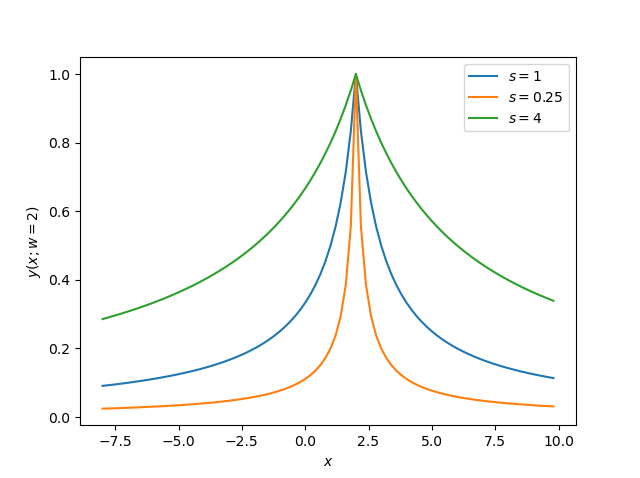
\includegraphics[scale=0.75]{img/zad_1.png}
    \caption{Ovisnost izlaza \textit{y} o \textit{s}}
    \label{zad1:img}
\end{figure}
Sa slike \ref{zad1:img} se jasno uočava da što je manji \textit{s}, to je manji izlaz \textit{y}, odnosno primjeri koji su udaljeniji od centroida \textit{w} će biti kažnjeni više za manje vrijednosti parametra \textit{s}. U slučaju kada neuron ima dva ulaza, tada će izlaz biti još striktniji, tj. primjeri će se općenito više kažnjavati što su dalje od centroida. Parametri \textit{s\textsubscript{1}} i \textit{s\textsubscript{2}} služe za skaliranje koordinata i ovisno radi li se o izduženosti na x ili y osi, parametri će imati manje, odnosno veće vrijednosti.

\chapter{Zadatak 2}
\begin{figure}[H]
    \centering
    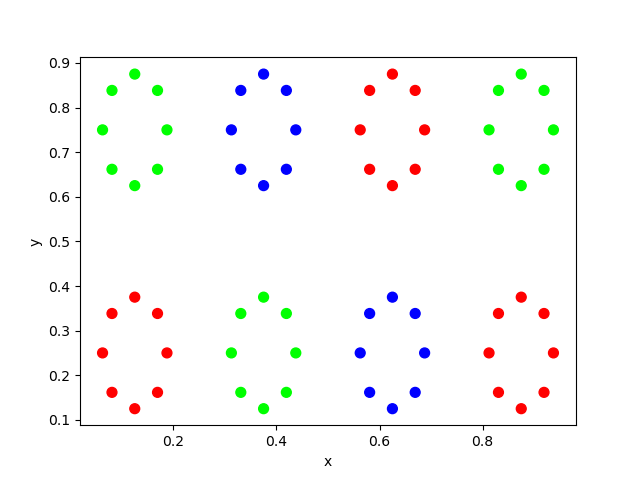
\includegraphics[scale=0.75]{img/zad_2.png}
    \caption[Caption for LOF]{Prikaz 2D podataka iz dataseta\footnotemark}
    \label{zad2:img}
\end{figure}
\footnotetext{Izrađeno pomoću programskog jezika \textit{Python} i biblioteke \textit{Matplotlib}.}
Slika \ref{zad2:img} jasno prikazuje kako su primjeri grupirani u 8 elipsa od kojih 3 crvene pripadaju razredu A, 3 zelene razredu B i 2 plave razredu C. Primjeri su linearno odvojivi. 

\chapter{Zadatak 3}
\begin{figure}[H]
    \centering
    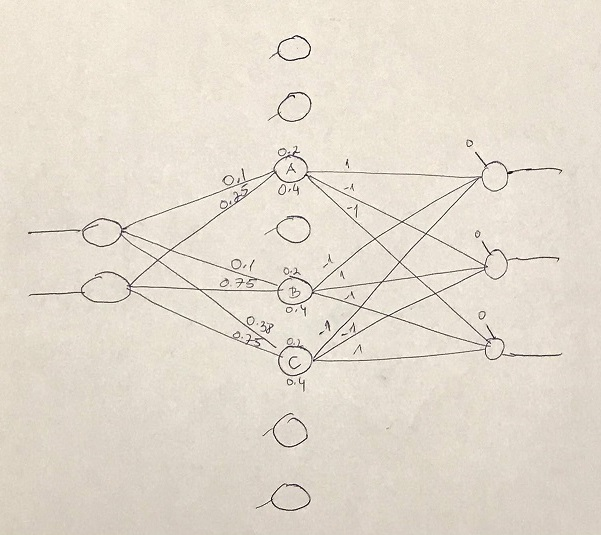
\includegraphics[scale=0.65]{img/zad_3.jpg}
    \caption{2x8x3 mreža}
    \label{zad3:img}
\end{figure}
Na slici \ref{zad3:img} prikazana je arhitektura 2x8x3 neuronske mreže gdje su, radi preglednosti, prikazani parametri samo za 3 nasumično odabrana neurona skrivenog sloja, koji su nazvani po željenim razredima, i za neurone izlaznog sloja. Težine skrivenog sloja sam odredio (odokativno pomoću slike \ref{zad2}) na temelju centroida, pa tako vrijednosti težina neurona A iznose 0.1 i 0.25, što predstavlja središte lijeve donje crvene elipse, vrijednosti težina neurona B iznose 0.1 i 0.75, što predstavlja središte lijeve gornje zelene elipse te vrijednosti težina neurona C iznose 0.38 i 0.75, što predstavlja središte prve gornje plave elipse. Parametre \textit{s\textsubscript{1}} i \textit{s\textsubscript{2}} sam postavio na 0.2, odnosno 0.4 jer po slici \ref{zad2:img} zaključujem da su skaliranja podjednaka s obzirom na pravilan izgled svake elipse. Također, parametar \textit{s\textsubscript{2}} je nešto veći jer su elipse malo izdužene po osi y. Težine izlaznog sloja sam postavio na 1, odnosno -1 zbog toga što one najbolje pokazuju koji neuron skrivenog sloja predstavlja koji razred. Valja napomenuti da neuroni skrivenog sloja generiraju brojeve koji su u intervalu $[0,1]$, stoga će se net vrijednost izlaznog neurona povećavati za pozitivne težine, dok će se za negativne smanjivati. Neuron sa najvećom net vrijednosti ćemo uzeti kao klasifikaciju uzorka.

\chapter{Zadatak 4}
\begin{figure}[H]
    \centering
    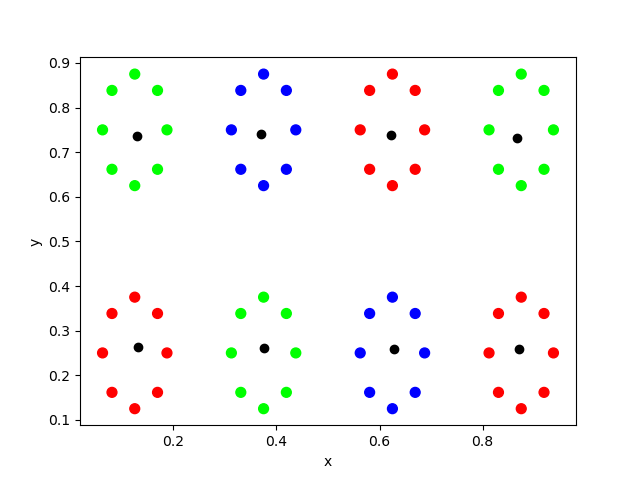
\includegraphics[scale=0.7]{img/zad_4.png}
    \caption[Caption for LOF]{Prikaz 2D podataka iz dataseta i centroida\footnotemark}
    \label{zad4:img}
\end{figure}
\footnotetext{Izrađeno pomoću programskog jezika \textit{Python} i biblioteke \textit{Matplotlib}.}

\begin{table}[H]
    \centering
    \begin{tabular}{|c c c c c|} 
        \hline
        n & w\textsubscript{1} & w\textsubscript{2} & s\textsubscript{1} & s\textsubscript{2} \\ [0.5ex] 
        \hline\hline
        \rowcolor{Red}
        1 & 0.87056693 & 0.25968479 & 0.11341864 & -0.19099131 \\
        \rowcolor{Red}
        2 & 0.1314665 & 0.2639499 & -0.12664145 & -0.20936459 \\
        \rowcolor{Green}
        3 & 0.1301023 & 0.73605907 & -0.16223074 & 0.27078076 \\
        \rowcolor{Green}
        4 & 0.8663112 & 0.7311553 & 0.15539173 & 0.2879704 \\
        \rowcolor{Blue}
        5 & 0.62806508 & 0.25909509 & 0.0926306 & 0.19161737 \\
        \rowcolor{Red}
        6 & 0.62241627 & 0.73905119 & 0.09878658 & -0.25807171 \\
        \rowcolor{Green}
        7 & 0.37528285 & 0.26203972 & -0.10859568 & 0.22590302 \\
        \rowcolor{Blue}
        8 & 0.36919078 & 0.74043638 & -0.08410955 & 0.22291554 \\ [1ex]
        \hline
    \end{tabular}
    \caption{Rezultati neurona tipa 1}
    \label{zad4:table1}
\end{table}

\begin{table}[H]
    \centering
    \begin{tabular}{|c c c c|} 
        \hline
        w\textsubscript{i} & n\textsubscript{1} & n\textsubscript{2} & n\textsubscript{3} \\ [0.5ex] 
        \hline\hline
        \rowcolor{Red}
        w\textsubscript{1} & 40.45028853 & -38.82630971 & -17.90848041 \\
        \rowcolor{Green}
        w\textsubscript{2} & -21.70054252 & 34.0055676 & -14.49969529 \\
        \rowcolor{Green}
        w\textsubscript{3} & -38.64338231 & 39.66207396 & -22.73612466 \\
        \rowcolor{Green}
        w\textsubscript{4} & -40.6041046 & 74.55624848 & -30.00203565 \\
        \rowcolor{Blue}
        w\textsubscript{5} & -7.65317838 & -58.3419473 & 69.27153891 \\
        \rowcolor{Blue}
        w\textsubscript{6} & -53.73290204 & -32.61985817 & 63.67829537 \\
        \rowcolor{Red}
        w\textsubscript{7} & 40.69039549 & -21.70882187 & -13.97546124 \\
        \rowcolor{Red}
        w\textsubscript{8} & 76.24550913 & -32.76116995 & -30.57446468 \\ [1ex]
        \hline
    \end{tabular}
    \caption{Rezultati neurona tipa 2}
    \label{zad4:table2}
\end{table}

U navedenim tablicama se nalaze eksperimentalni rezultati za neuronsku mreže arhitekture 2x8x3 koju smo u trećem zadatku teorijski obradili. Tablica \ref{zad4:table1} predstavlja parametre neurona tipa 1 i možemo vidjeti da težine predstavljaju centroid dotične elipse, što je i označeno prikladnom bojom u istoj, dok parametri \textit{s} predstavljaju koliko je centroid udaljen od elipse po x osi, odnosno po y osi i također uočavamo da je parametar \textit{s}\textsubscript{2} nešto veće apsolutne vrijednosti zbog izduženosti elipse u smjeru osi y.

Tablica \ref{zad4:table2} predstavlja težine (bez pomaknuća) neurona tipa 2 i također možemo vidjeti da je teorija trećeg zadatka potvrđena. U prvom retku možemo vidjeti da postoji jedna pozitivna težina i dvije negativne pa se da zaključiti da neuron iz kojeg izlaze dotične težine, dakle neurona tipa 1, predstavlja razred označen crvenom bojom, tj. razred A. Analogno se pokazuje i za ostale rezultate.

\chapter{Zadatak 5}
\begin{figure}[H]
    \centering
    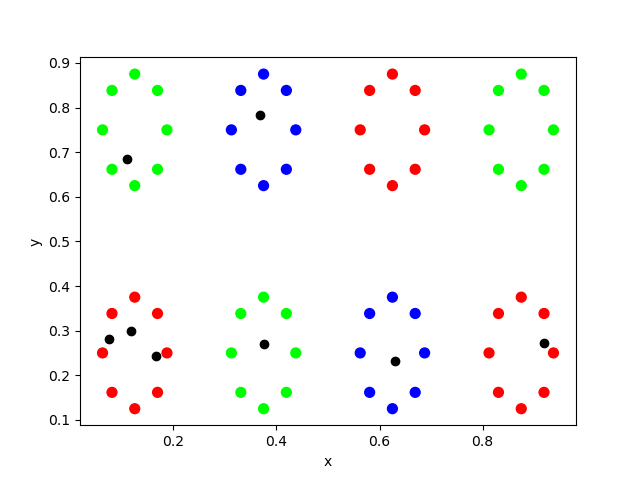
\includegraphics[scale=0.7]{img/zad_5.png}
    \caption[Caption for LOF]{Prikaz 2D podataka iz dataseta i centroida\footnotemark}
    \label{zad5:img}
\end{figure}
\footnotetext{Izrađeno pomoću programskog jezika \textit{Python} i biblioteke \textit{Matplotlib}.}

\begin{table}[H]
    \centering
    \begin{tabular}{|c c c c c|} 
        \hline
        n & w\textsubscript{1} & w\textsubscript{2} & s\textsubscript{1} & s\textsubscript{2} \\ [0.5ex] 
        \hline\hline
        \rowcolor{Red}
        1 & 0.9195599 & 0.27235955 & 0.12174026 & 0.03232097 \\
        \rowcolor{Blue}
        2 & 0.36798174 & 0.78226241 & 0.10437182 & -0.44402148 \\
        \rowcolor{Green}
        3 & 0.3751542 & 0.26965979 & 0.14072831 & -0.20409056 \\
        \rowcolor{Blue}
        4 & 0.63004829 & 0.23219823 & 0.10609551 & -0.22998608 \\
        \rowcolor{Red}
        5 & 0.16582354 & 0.24307991 & -0.03865407 & -0.14058263 \\
        \rowcolor{Red}
        6 & 0.11751811 & 0.29809988 & 0.09172907 & 1.03435842 \\
        \rowcolor{Green}
        7 & 0.10930424 & 0.68436357 & -0.11396174 & 0.12717252 \\
        \rowcolor{Red}
        8 & 0.07466577 & 0.28177913 & -0.0645295 & -1.77172434 \\ [1ex]
        \hline
    \end{tabular}
    \caption{Rezultati neurona tipa 1}
    \label{zad5:table}
\end{table}

\chapter{Zadatak 6}
\begin{figure}[H]
    \centering
    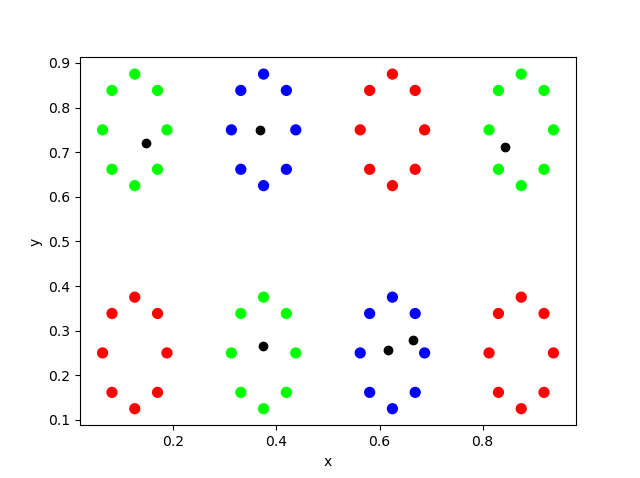
\includegraphics[scale=0.7]{img/zad_6.png}
    \caption[Caption for LOF]{Prikaz 2D podataka iz dataseta i centroida\footnotemark}
    \label{zad6:img}
\end{figure}
\footnotetext{Izrađeno pomoću programskog jezika \textit{Python} i biblioteke \textit{Matplotlib}.}

\begin{table}[H]
    \centering
    \begin{tabular}{|c c c c c|} 
        \hline
        n & w\textsubscript{1} & w\textsubscript{2} & s\textsubscript{1} & s\textsubscript{2} \\ [0.5ex] 
        \hline\hline
        \rowcolor{Blue}
        1 & 0.61583717 & 0.25675516 & 0.10189873 & -0.14831607 \\
        \rowcolor{Green}
        2 & 0.14760045 & 0.72062042 & 0.17817954 & 0.7916723 \\
        \rowcolor{Green}
        3 & 0.84346026 & 0.7114165 & 0.32701894 & 0.37441321 \\
        \rowcolor{Blue}
        4 & 0.36746019 & 0.75021939 & -0.08642462 & 0.45354458 \\
        \rowcolor{Blue}
        5 & 0.66560164 & 0.27987725 & -0.05899077 & 0.50943645 \\
        \rowcolor{Green}
        6 & 0.37451733 & 0.26587057 & 0.19097825 & -0.25518653 \\ [1ex]
        \hline
    \end{tabular}
    \caption{Rezultati neurona tipa 1}
    \label{zad6:table}
\end{table}

\bibliography{literatura}
\bibliographystyle{fer}
\nocite{*}

\end{document}
